\documentclass[tikz,border=10pt]{standalone}
\usepackage{tkz-euclide} % 引入几何增强宏包，简化坐标计算

\begin{document}
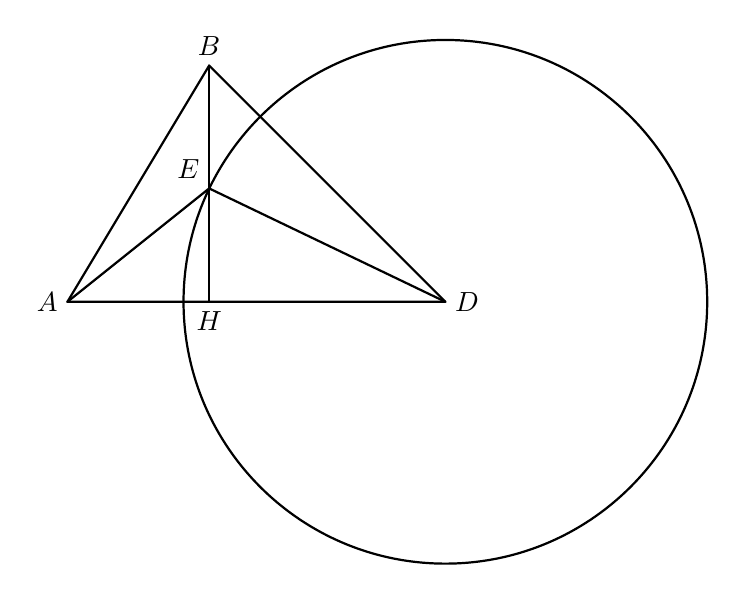
\begin{tikzpicture}[line join=round, line cap=round, scale=1.2]
    % 1. 定义基本参数（可根据实际题目数值调整）
    \coordinate (A) at (0, 0);          % 点 A
    \coordinate (D) at (4, 0);          % 点 D
    \coordinate (H) at (1.5, 0);        % 垂足 H 位于 AD 上
    \coordinate (B) at (1.5, 2.5);      % 顶点 B，垂直于 H
    
    % 2. 计算圆与辅助点
    % 设圆心为 D，半径为 DE 的长度。根据原图 E 位于 BH 上。
    \coordinate (E) at (1.5, 1.2);      % 垂线上的特殊点 E
    
    % 计算圆的半径 (D 到 E 的距离)
    \path let \p1 = ($(E)-(D)$) in \pgfextra{\pgfmathsetmacro{\rad}{veclen(\x1,\y1)}\xdef\radius{\rad}};

    % 3. 绘制图形中心元素
    % 绘制大三角形 ABD
    \draw[thick] (A) -- (B) -- (D) -- cycle;
    
    % 绘制垂线 BH
    \draw[thick] (B) -- (H);
    
    % 绘制连接线 AE 和 DE
    \draw[thick] (A) -- (E) -- (D);
    
    % 绘制以 D 为圆心经过 E 的圆
    \draw[thick] (D) circle (\radius pt);

    % 4. 标注文本（使用 auto 自动定位或手动偏移）
    \node[left] at (A) {$A$};
    \node[right] at (D) {$D$};
    \node[above] at (B) {$B$};
    \node[below] at (H) {$H$};
    \node[above left] at (E) {$E$};
    
    % 5. 绘制直角符号 (可选)
    %\draw (H) ++(0,0.2) -- ++(0.2,0) -- ++(0,-0.2);

\end{tikzpicture}
\end{document}